% ------------------------------------------------------------------------ %
% !TEX encoding = UTF-8
% !TEX TS-program = pdflatex
% !TEX root = ../Project.tex
% !TEX spellcheck = en-EN
% ------------------------------------------------------------------------ %
%
% ------------------------------------------------------------------------ %
% 	CHAPTER TITLE
% ------------------------------------------------------------------------ %
%
\chapter{Graphical representations}
%
%
% ------------------------------------------------------------------------ %
%
\section{C-IDM}
In this schema are indentified Single topics (Who we are, News, Contact us, Help us, F.A.Q.), Multiple topics (Event, Location, Service, People), their groups, relevant relations and cardinalities.
%
\begin{figure}[h]
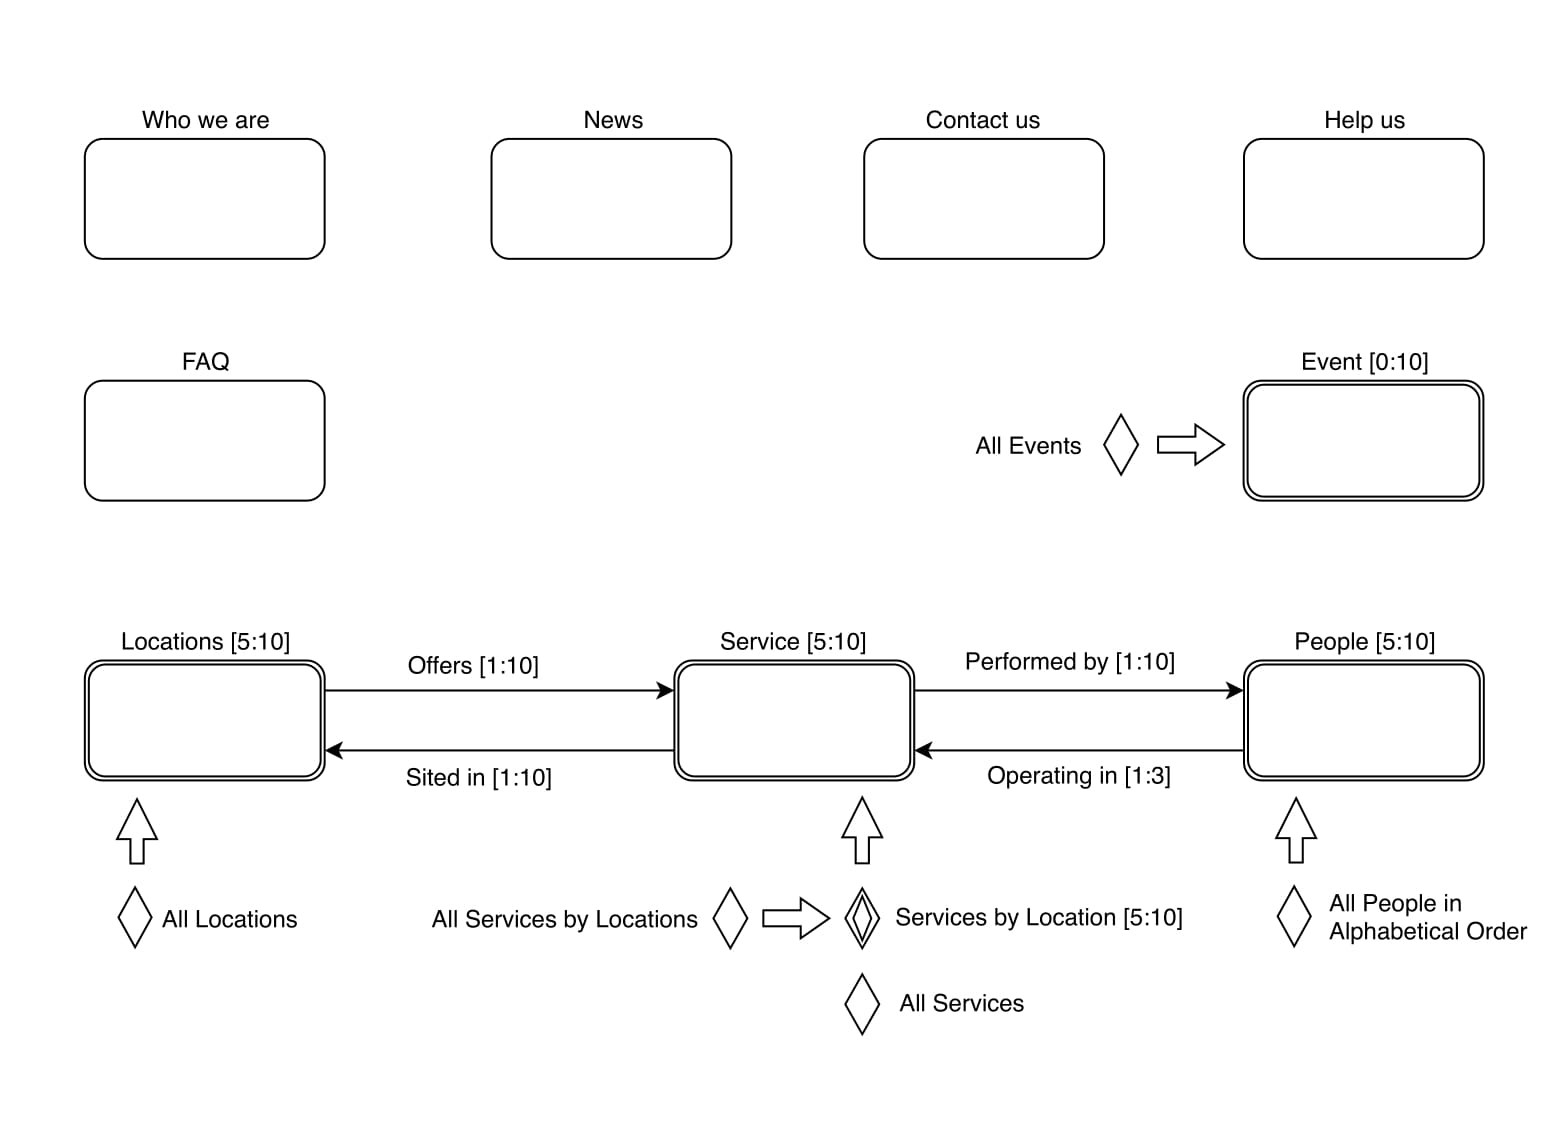
\includegraphics[width=1.03\textwidth, center]{MainMatter/images/C-IDM.jpg}
\caption{C-IDM}
\label{fig:figure1}
\end{figure}
\FloatBarrier
% ------------------------------------------------------------------------ %
%
\section{L-IDM}
On the logical level dialogue acts are added for every topic, while groups and multiple groups translates into introductory dialogue acts. On the news topic we decided separate internal news of the association from other external news that could interest the world of disability associations and to add here a category of news which are more related to logistical informations called important announcements. In the contact us topic we included every information related to generic association contacts, including locations contacts and position, while the contacts related to people working in the association are left in their topic. Also we added here the helper form to contact the association directly from the site. In the help us topic, after general explenation on how to help, we distinguished two kind of donations, money and goods. In the event topic we choose to put a photogallery of past editions because it's the best way to understand how the event is going to be, togather with an optional dialogue act on partecipation requirements that could be used in closed number events. Who we are, Location, Service and Person are intended to present what the association can offer to the interested public.
%
\begin{figure}[h]
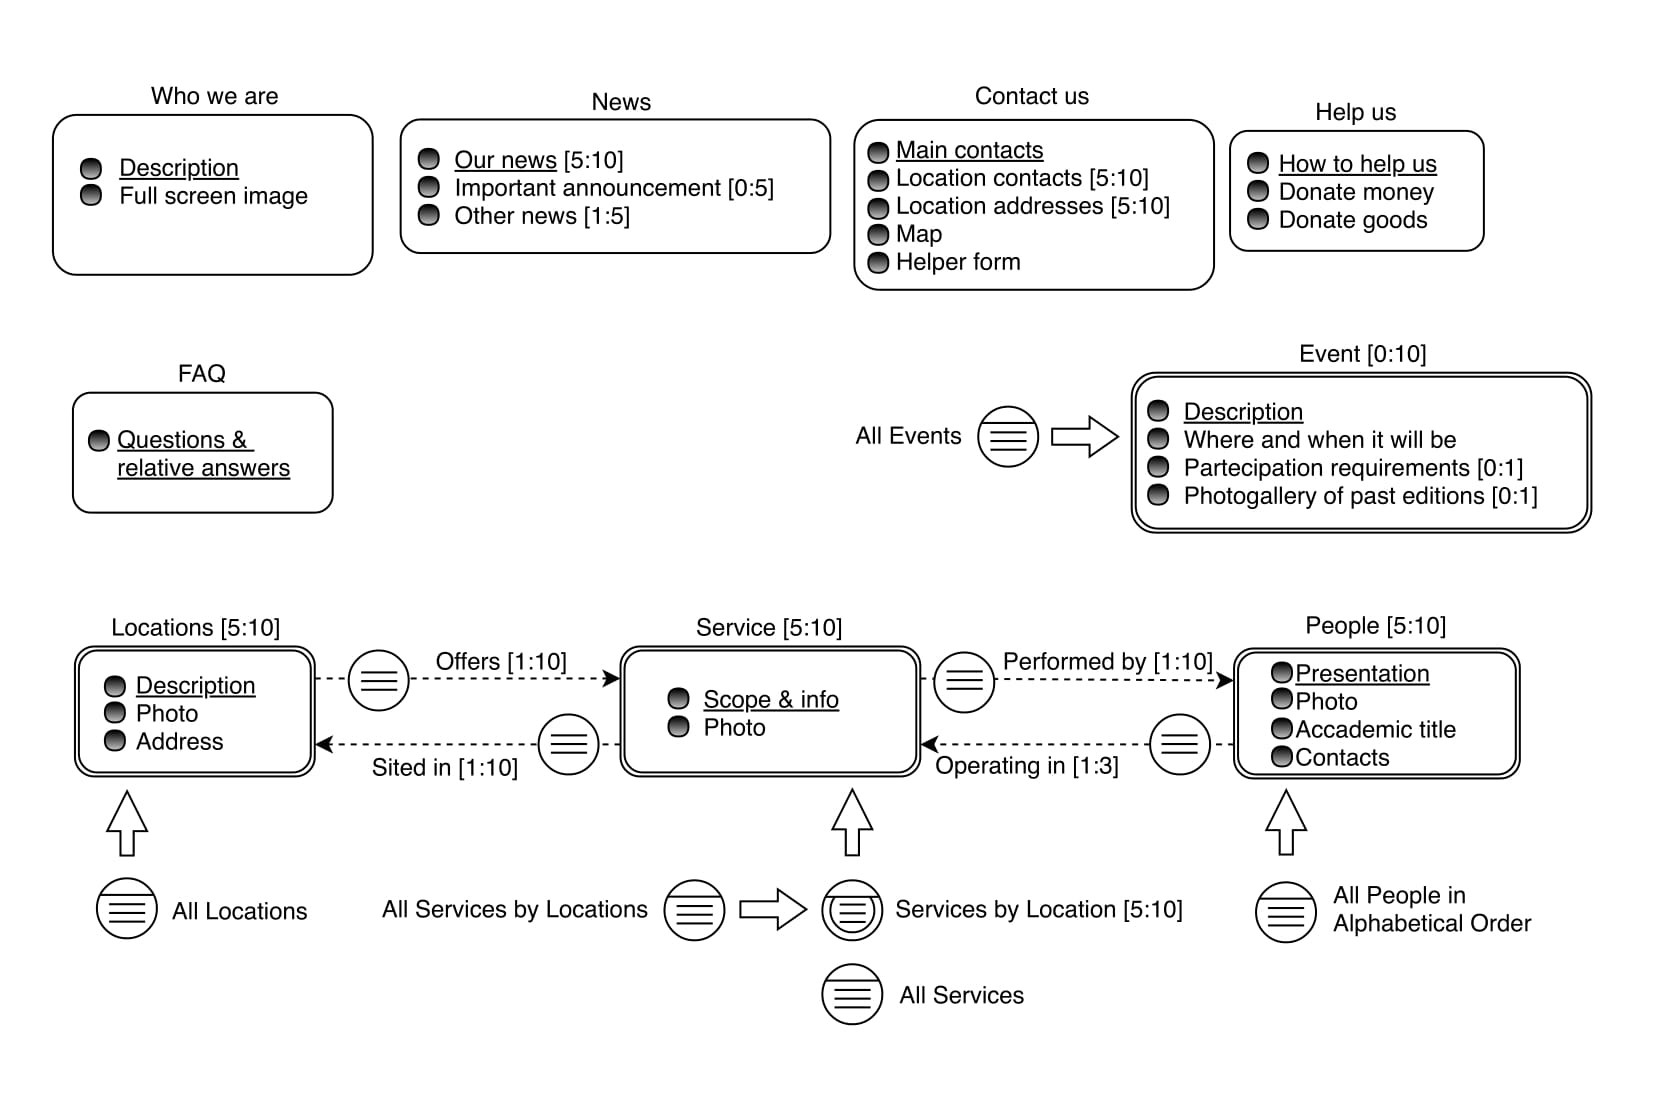
\includegraphics[width=1.5\textwidth, center]{MainMatter/images/L-IDM.jpg}
\caption{L-IDM}
\label{fig:figure2}
\end{figure}
\newpage
% ------------------------------------------------------------------------ %
%
\section{P-IDM}
%
In the end we distributed the dialogue acts, relevant relations and groups into pages and we defined the links between them. All the topics include only one page, in fact we did't need to make separate pages for different dialogue acts because most of them are small and with the latest technologies in web design it is possible to fit in a dynamic way many pieces of information in one page. From now one I will use topic and page as synonyms, but it only applys for the reason above, being them two different concepts. Talking about pages we decided to merge Person, Service and Location topic pages with their respective transition pages and links, and to use dynamic introductory pages for the all services group and the multiple group of services by location connected by structural links. Moreover all groups will have group links to cycle through the pages, as highlighted by the grand tour pattern. To conclude this section, landmarks will be the same in every page.
\begin{figure}[h]
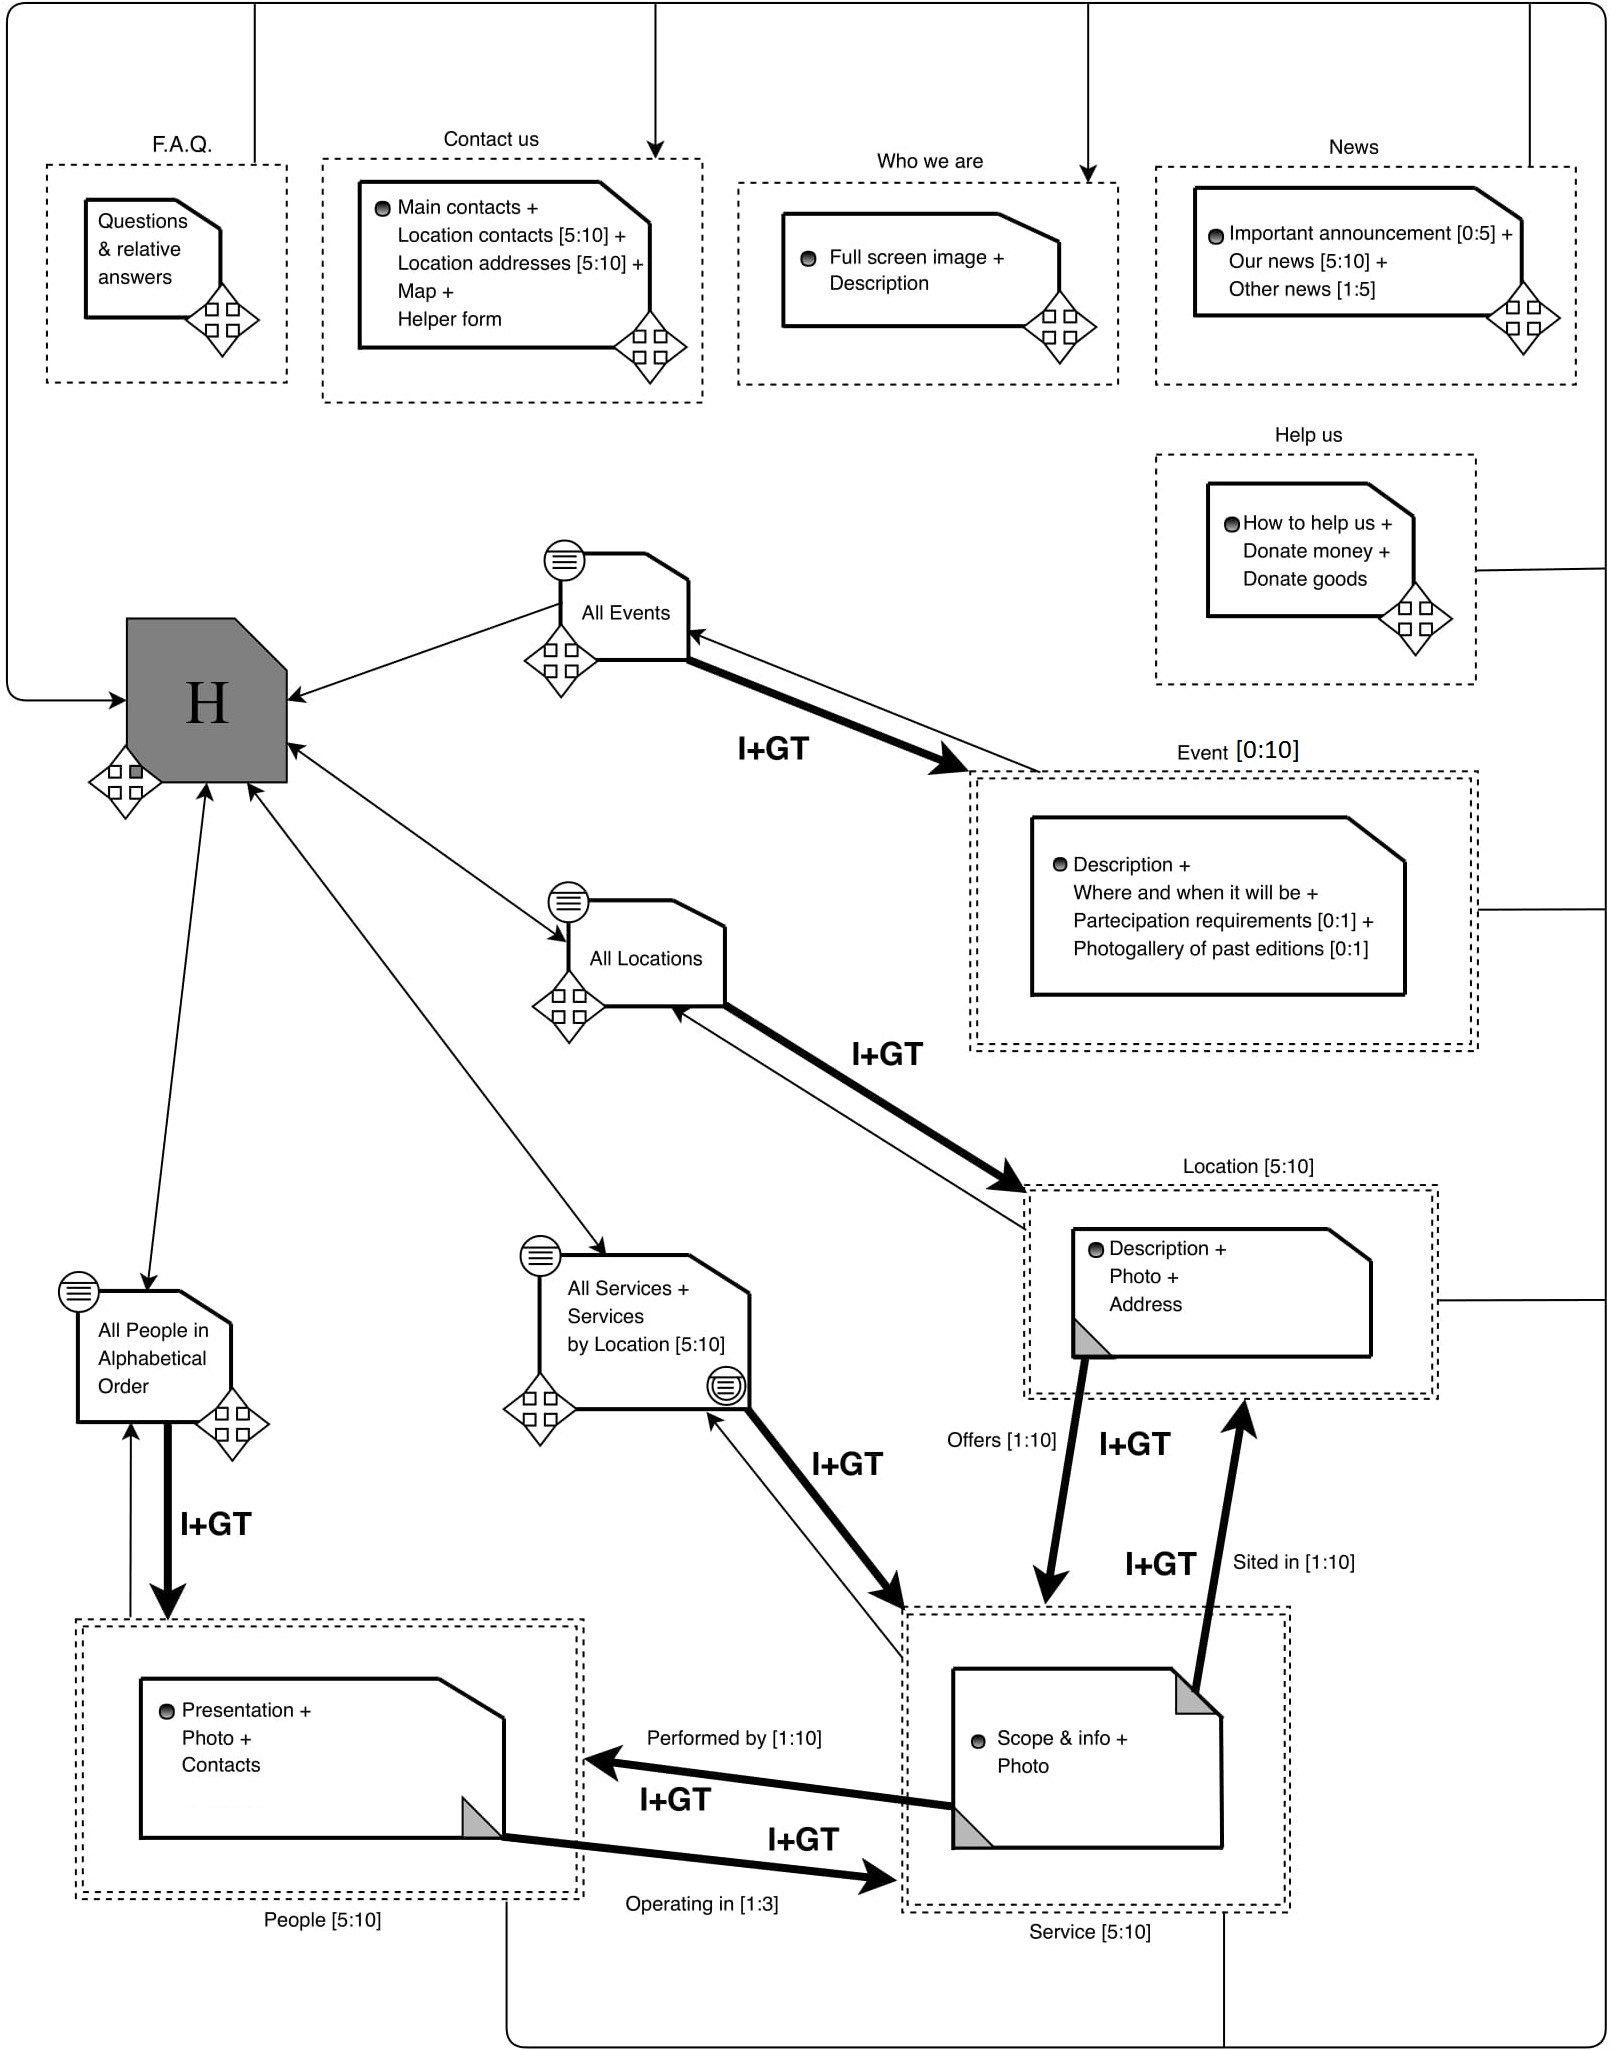
\includegraphics[width=1.17 \textwidth, center]{MainMatter/images/P-IDM.jpg}
\caption{P-IDM}
\label{fig:figure3}
\end{figure}
% -----------------------------END------------------------------------- %